\documentclass{ximera}

\title{Multivariable Optimization}
\author{Zack Reed}

\begin{document}
\begin{abstract}
In this activity we explore optimization in multivariable settings, starting with gradient descent as a modern computational approach, then examining the mathematical foundations through gradients, critical points, and the Hessian matrix.
\end{abstract}
\maketitle

\section*{Introduction: Why Optimize?}

Optimization is everywhere in modern applications:
\begin{itemize}
    \item Machine learning models minimize error functions
    \item Engineers maximize efficiency while minimizing cost
    \item Physicists find states of minimum energy
    \item Economists maximize profit while minimizing waste
\end{itemize}

In single-variable calculus, we found extrema by setting $f'(x)=0$ and testing with the second derivative. In multivariable settings, we need new tools!

\begin{problem}
Review: In single-variable calculus, to find the minimum of $f(x) = x^2 - 4x + 5$, we would:

\begin{enumerate}
    \item Find the critical point by solving $f'(x) = \answer{2x-4} = 0$, giving $x = \answer{2}$.
    \item Check the second derivative: $f''(x) = \answer{2}$.
    \item Since $f''(2) > 0$, we conclude this is a \wordChoice{\choice{maximum}\choice[correct]{minimum}\choice{saddle point}}.
    \item The minimum value is $f(2) = \answer{1}$.
\end{enumerate}

\begin{feedback}
    This process extends to multivariable functions, but with new twists! We'll need gradients instead of derivatives, and the Hessian matrix instead of the second derivative.
\end{feedback}
\end{problem}

Let's first explore this process for the first derivative in single-variable calculus.

\begin{problem}
Explore the following applet to see how the first derivative tests works

\begin{expandable}{stuff}{GeoGebra Instructions}
    Read the text on screen and advance the animation by clicking the buttons (in red or black text) to view new text, tangent lines, and portions of the graph. Use the reset button at the bottom left to start over.
\end{expandable}
\begin{center}
\geogebra{ebuvppdr}{757}{611}
\end{center}

After exploring the applet, identify what you observed (Select All that are true):
\begin{selectAll}
    \choice[correct]{When $f'(x) > 0$, the graph is increasing}
    \choice[correct]{When $f'(x) < 0$, the graph is decreasing}
    \choice{When $f'(x) = 0$, the graph is always a maximum or minimum}
    \choice{The first derivative measures the concavity of the function}
    \choice[correct]{At points where $f'(x) = 0$, there may be a local maximum or minimum, but further testing is needed.}
\end{selectAll}

\begin{feedback}
The first derivative measures the function's rates of change, telling us when it increases and decreases. If the derivative is zero, there is possible a local max or min, but you need to test around the point to be sure.
\end{feedback}
\end{problem}

\begin{problem}
Now explore the implications of the second derivative in greater depth in the following applet.

\begin{expandable}{stuff}{GeoGebra Instructions}
    Read the text on screen and advance the animation by clicking the buttons (in red or black text) to view new text, tangent lines, and portions of the graph. Use the reset button at the bottom left to start over.
\end{expandable}

\begin{center}
\geogebra{uervaqau}{757}{611}
\end{center}

After exploring the applet, identify what you observed (Select All that are true):
\begin{selectAll}
    \choice[correct]{When $f''(x)  > 0$, the graph bends upward}
    \choice[correct]{When $f''(x) < 0$, the graph bends downward}
    \choice{When $f''(x) = 0$, the graph is always a straight line}
    \choice{The second derivative measures the slope of the function}
\end{selectAll}

\begin{feedback}
The second derivative measures how the first derivative (slope) changes, not the slope itself. This rate of change of slope is what we call concavity.
\end{feedback}
\end{problem}


\subsection*{Generalizing to Higher Dimensions: From First Derivatives to The Gradient Vector}

\begin{definition}
For a function $f(x,y)$, the \textbf{gradient} is the vector of partial derivatives:
$$\nabla f = \left\langle \frac{\partial f}{\partial x}, \frac{\partial f}{\partial y} \right\rangle$$
\end{definition}

In single-variable calculus, we found points where $f'(x) = 0$ to locate possible min and max values. This was because nonzero derivatives meant the function \wordChoice{\choice{possibly increased or decreased}\choice[correct]{had to either increase or decrease}\choice{was constant}} at that point.

Similarly, in multivariable calculus, if the gradient $\nabla f$ is nonzero at a point, then the function \wordChoice{\choice{possibly increases or decreases}\choice[correct]{must either increase or decrease}\choice{is constant}} in some direction at that point. This is because the directional derivative \wordChoice{\choice{is independent of the gradient}\choice[correct]{depends on a dot product with the gradient}}.

So, the only possible locations for maximum or minimum values are \wordChoice{\choice{where the gradient is nonzero}\choice[correct]{where the gradient is zero}}.

\begin{definition}
A point $(x_0, y_0)$ is a \textbf{critical point} of $f(x,y)$ if:
$$\nabla f(x_0, y_0) = \langle 0, 0 \rangle$$.

This means:
$$\frac{\partial f}{\partial x}(x_0, y_0) = 0 \quad \text{and} \quad \frac{\partial f}{\partial y}(x_0, y_0) = 0$$
\end{definition}

\begin{remark}
Technically, we also care about when the derivative (or graident) is undefined, but for this activity we will focus on where it is zero.
\end{remark}

\begin{problem}
Why do we care about critical points?

\begin{multipleChoice}
    \choice{They are always minima}
    \choice{They are always maxima}
    \choice[correct]{Local extrema must occur at critical points (if they exist in the interior)}
    \choice{The function is undefined at critical points}
\end{multipleChoice}
\end{problem}

\begin{problem}
Find the critical points of $f(x,y) = x^2 + y^2 - 4x + 6y + 5$.

First, compute the partial derivatives:
$$\frac{\partial f}{\partial x} = \answer{2x - 4}$$
$$\frac{\partial f}{\partial y} = \answer{2y + 6}$$

Set them equal to zero and solve:
$$2x - 4 = 0 \Rightarrow x = \answer{2}$$
$$2y + 6 = 0 \Rightarrow y = \answer{-3}$$

The critical point is $(\answer{2}, \answer{-3})$.

This is a paraboloid (bowl shape). Based on the shape, we can guess this critical point is a \wordChoice{\choice{maximum}\choice[correct]{minimum}\choice{saddle point}}.

%plot the function
\begin{center}
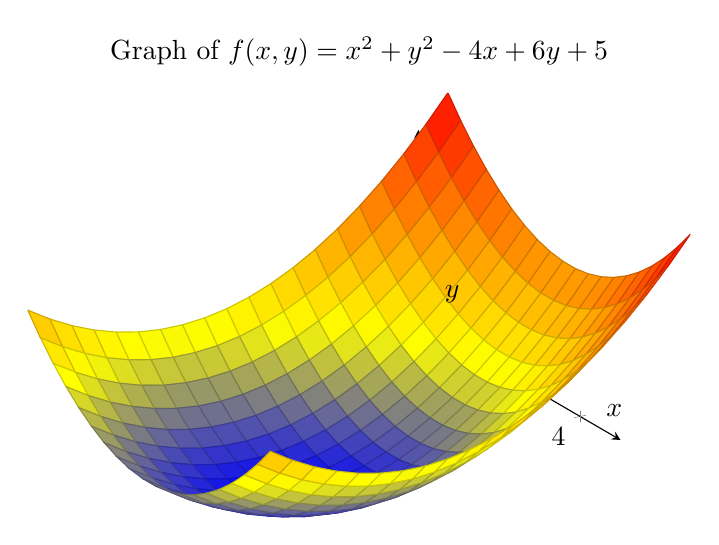
\begin{tikzpicture}
    \begin{axis}[
        axis lines = center,
        xlabel = $x$,
        ylabel = {$y$},
        title = {Graph of $f(x,y) = x^2 + y^2 - 4x + 6y + 5$},
        width=10cm,
        height=8cm,
        grid=major,
        view={60}{30},
    ]
    \addplot3[surf,domain=-1:5,y domain=-5:1,samples=20] {x ^2 + y ^2 - 4*x + 6*y + 5};
    \end{axis}
\end{tikzpicture}
\end{center}

\end{problem}

\section*{Caution: Not All Critical Points are Extrema!}

In single-variable calculus, we weren't always guaranteed a max or min at critical points. The same is true in multivariable calculus.

\begin{problem}
Let's first review this issue with the function $f(x) = x^3$.

\begin{center}
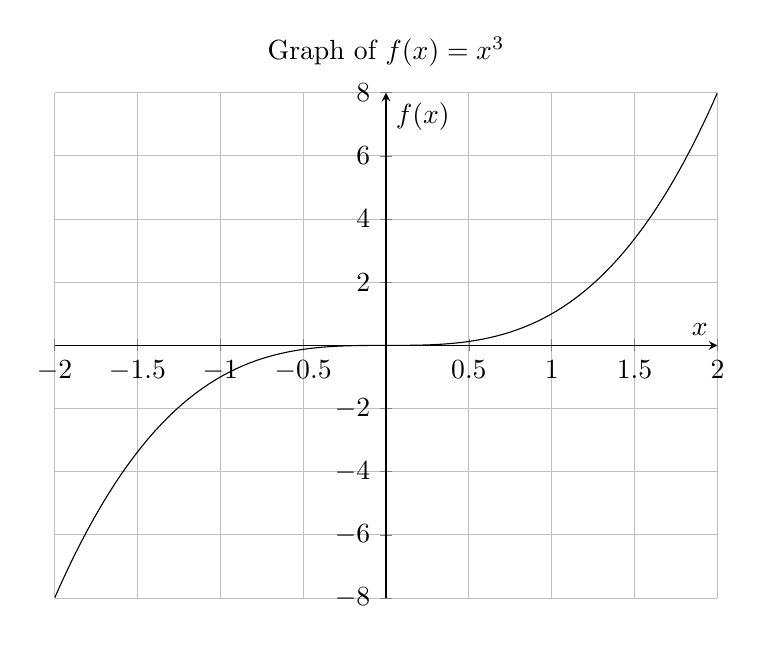
\begin{tikzpicture}
    \begin{axis}[
        axis lines = center,
        xlabel = $x$,
        ylabel = {$f(x)$},
        title = {Graph of $f(x) = x^3$},
        width=10cm,
        height=8cm,
        grid=major,
    ]
    \addplot[domain=-2:2,samples=100] {x ^3};
    \end{axis}
\end{tikzpicture}
\end{center}

Even though the derivative is zero at $x=0$, if you move forward in $x$, the function \wordChoice{\choice{decreases}\choice[correct]{increases}}; and if you move backward in $x$, the function \wordChoice{\choice{decreases}\choice[correct]{increases}}. So there \wordChoice{\choice[correct]{is no}\choice{is a}} max or min at this critical point!
\end{problem}


\begin{problem}
Find the critical points of $f(x,y) = x^2 - y^2$.

The partial derivatives are:
$$\frac{\partial f}{\partial x} = \answer{2x}$$
$$\frac{\partial f}{\partial y} = \answer{-2y}$$

Setting both equal to zero: $x = \answer{0}$ and $y = \answer{0}$.

The critical point is $(\answer{0}, \answer{0})$.

This function looks like a saddle at the origin - it curves up in one direction and down in another. The critical point is neither a minimum nor a maximum! This is called a saddle point.

\end{problem}

\begin{center}
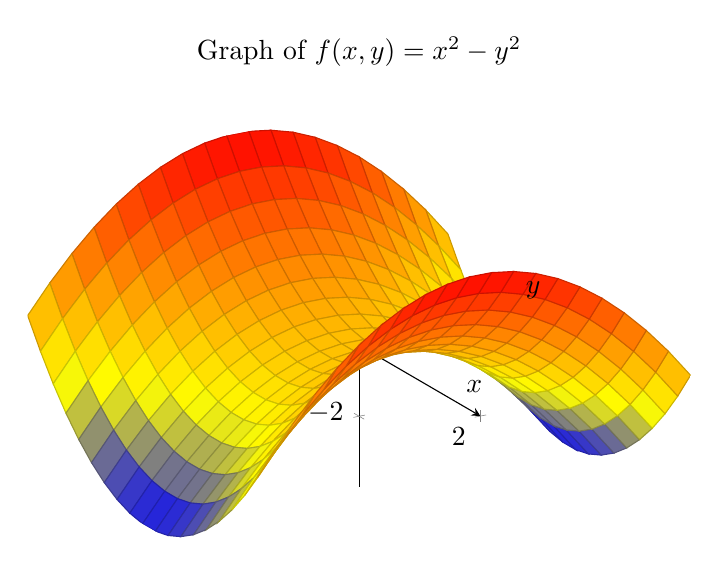
\begin{tikzpicture}
    \begin{axis}[
        axis lines = center,
        xlabel = $x$,
        ylabel = {$y$},
        title = {Graph of $f(x,y) = x^2 - y^2$},
        width=10cm,
        height=8cm,
        grid=major,
        view={60}{30},
    ]
    \addplot3[surf,domain=-2:2,y domain=-2:2,samples=20] {x ^2 - y ^2};
    \end{axis}
\end{tikzpicture}
\end{center}


\end{document}
